%! Author = tstreule

\section{Fluorescent Probes}
%%%%%%%%%%%%%%%%%%%%%%%%%%%%%%%%%%%%%%%%%%%%%%%%%%%%%%
%%%%%%%%%%%%%%%%%%%%%%%%%%%%%%%%%%%%%%%%%%%%%%%%%%%%%%
\subsection{Fluorescence Statistics}
%
\textbf{Photobleaching}: A fluorescent molecule can emit a limited \#photons by excitation before it irreversibly converts to a non-fluorescent molecule.

\begin{minipage}{.3\columnwidth}
    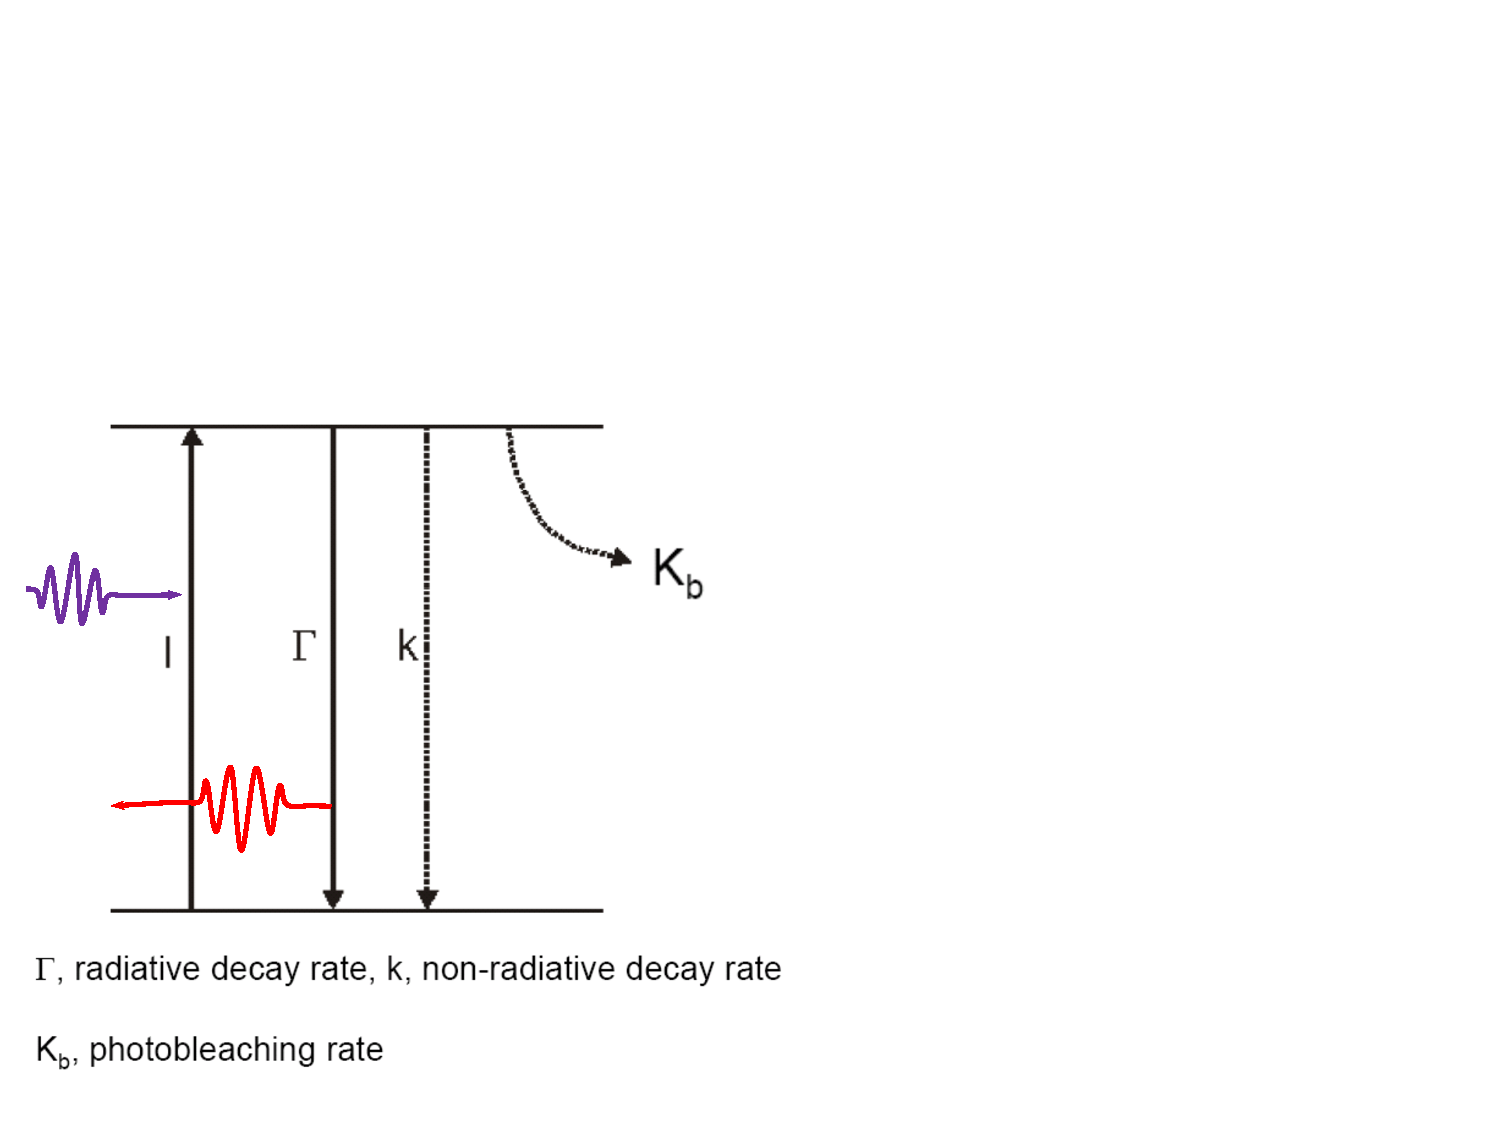
\includegraphics[width=.9\columnwidth]{Fluorescence_Statistics}
\end{minipage}%
\begin{minipage}{.7\columnwidth}
    \formula{\textbf{Quant. Yield}}{Q = \frac{\Gamma}{\Gamma+k+K_b} \sim 0-98\%}
    \hfill (Efficiency)
    \formbox{Fluorescence \textbf{Lifetime}}{\tau = \frac{1}{\Gamma+k+K_b} \sim \unit[1]{ns}}
    \vspace{1mm}

    Fluorescence emission is a statistical process that is characterized by exponential decays.
    \formula{Molecules in \textit{excited} state}{\deriv{N_e}{t} = -\left(\frac{1}{\tau_1}+\ldots+\frac{1}{\tau_n}\right) N_e}
\end{minipage}
%%%%%%%%%%%%%%%%%%%%%%%%%%%%%%%%%%%%%%%%%%%%%%%%%%%%%%
\columnbreak
\subsection{FRET \textnormal{-- Fluorescence Resonance Energy Transfer}}
%
\begin{minipage}{.25\columnwidth}
    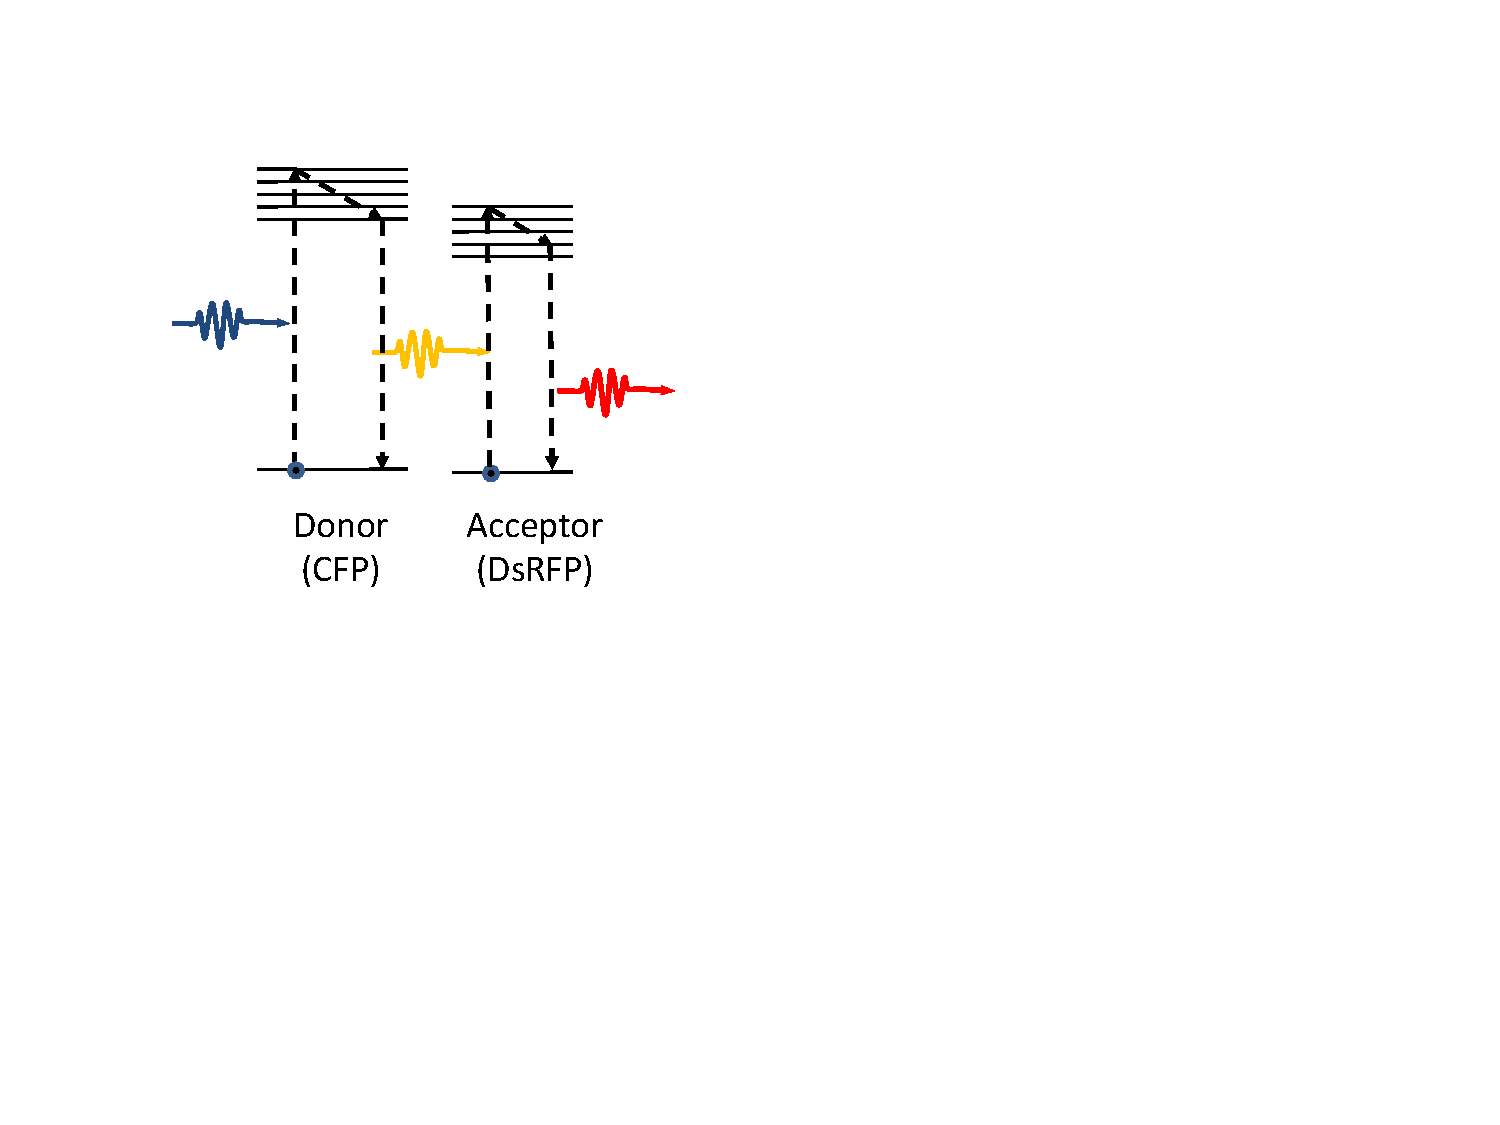
\includegraphics[width=.9\columnwidth]{Fluorescence_FRET}
\end{minipage}%
\begin{minipage}{.75\columnwidth}
    Seeing a different $\lambda\ped{emission}$ tells us that two molecules are close.
    \formbox{Efficiency}{E = \frac{R_0^2}{R_0^2+r^6} = 1\!-\!\frac{\tau\ped{DA}}{\tau\ped{D}} = 1\!-\!\frac{I\ped{DA}}{I\ped{D}}}
    where
    \formtex{$\tau\ped{D(A)}$, $I\ped{D(A)}$}{Lifetime/Intensity of donor emission}
    
    \formtex{~}{in the absence/presence of acceptor.}
\end{minipage}
%%%%%%%%%%%%%%%%%%%%%%%%%%%%%%%%%%%%%%%%%%%%%%%%%%%%%%
\subsection{Calcium Imaging \textnormal{\hfill $\to$ too slow for $t$ dependency meas.}}
%
Calcium ion cannot be visualized/tagged directly:
$\to$
Design molecules with optical properties that change upon calcium binding.

\begin{minipage}{.23\columnwidth}
    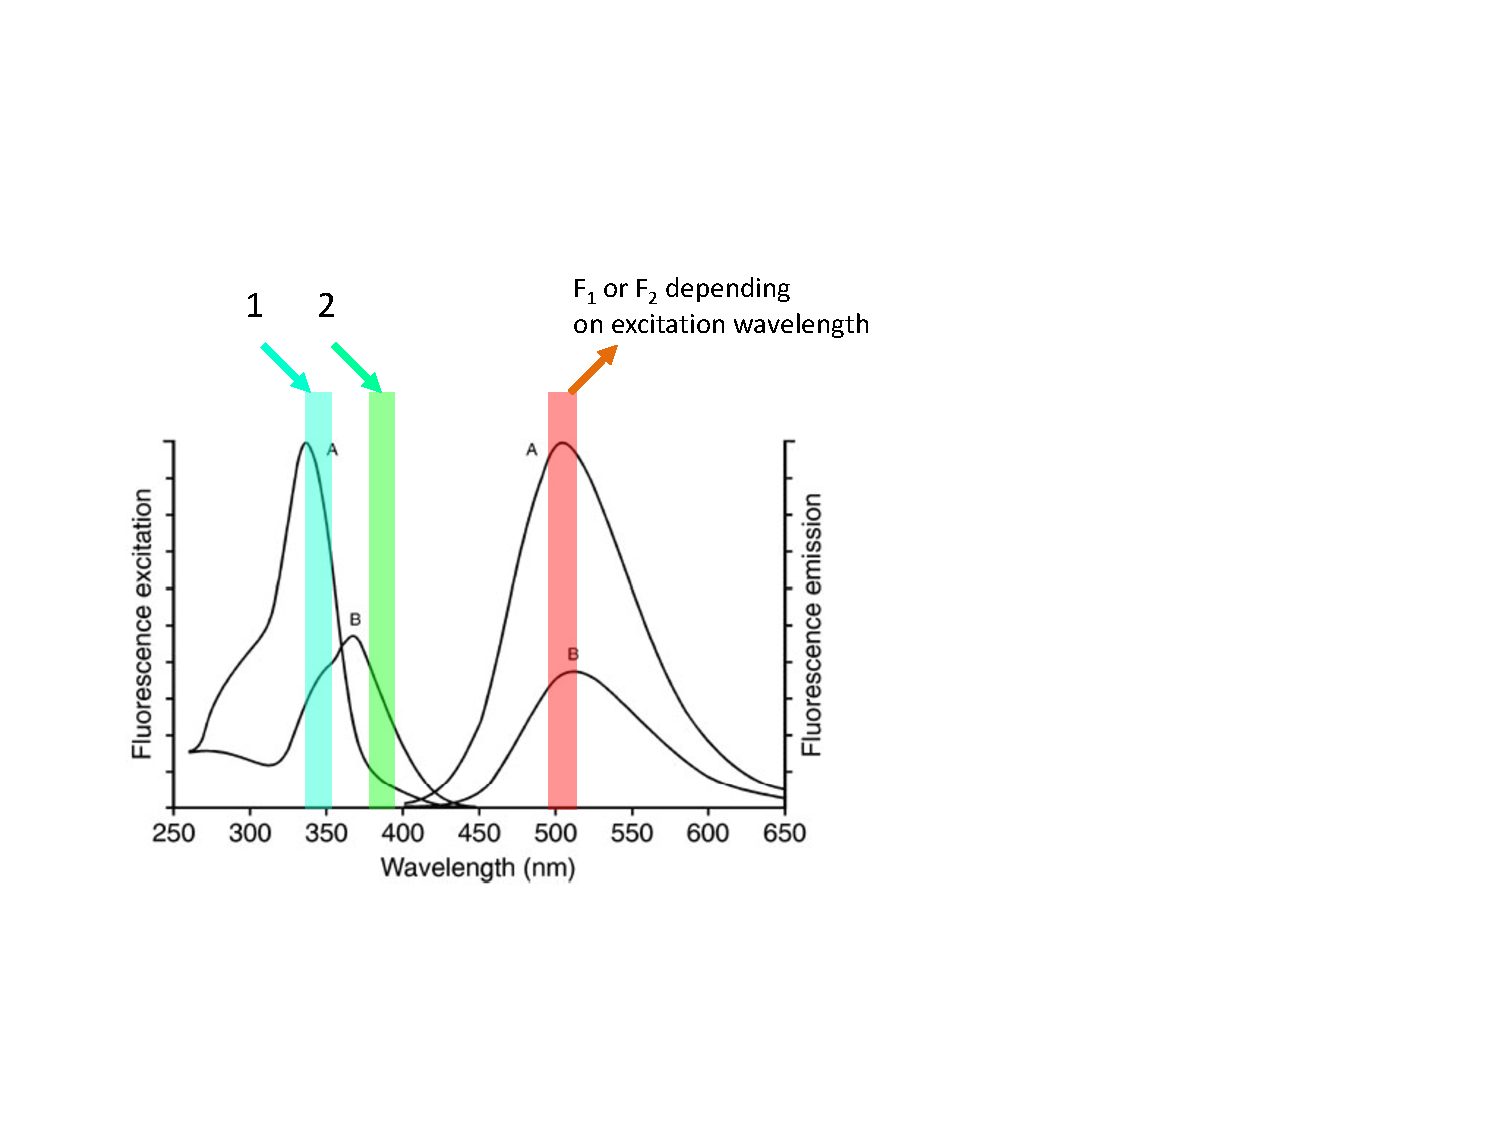
\includegraphics[width=\columnwidth]{Fluorescence_Calcium_Imaging}
\end{minipage}%
\hspace{\columnsep}%
\begin{minipage}{.77\columnwidth-\columnsep}
    \textbf{Single \& dual wavelength measurements}: 
    \formbox{Concentration}{[\ce{Ca^{2+}}]_i = K\ped{d,eff} \frac{R-R\ped{min}}{R\ped{max}-R}}
    where
    \formula{for single}{\scriptstyle R\equiv F \text{ and } K\ped{d,eff} = \frac{[\ce{Ca^{2+}}]_i \times(F\ped{max}-F)}{F-F\ped{min}}}
    \formula{for dual.}{R=F_1/F_2}
    \qquad ($F$: fluorescence)
%
%		where $R=F_1/F_2$ for dual wavelength and $R\equiv F$ and $K\ped{d,eff} = \frac{[\ce{Ca^{2+}}]_i \times(F\ped{max}-F)}{F-F\ped{min}}$ for single wavelength
\end{minipage}

The binding of \ce{Ca^{2+}} leads to\ldots
\begin{itemize}
    \item change in fluorescence \textbf{intensity} but not wavelength change
    \item a \textbf{shift} in excitation (and/or emission) peaks (``dual wavelength'')
    \item changes in fluor. resonance energy transfer (\textbf{FRET}) \& life time
\end{itemize}
%%%%%%%%%%%%%%%%%%%%%%%%%%%%%%%%%%%%%%%%%%%%%%%%%%%%%%
\subsubsection{Delivery of Calcium Indicators}
%
\formtex{\textbf{Loading cells}}{Once the molecule got cleaved (spalten), it}
\formtex{~}{cannot go out and gets fluorescent.}

\formtex{Introduce \textbf{fluoresc.}}{Proteins change emission rate when \ce{Ca} binds.}
\formtex{\textbf{proteins} or (natural)}{Relative change ($\Delta F/F$) in fluorescence}
\formtex{\textbf{FRET proteins}}{emission of EGFP can then be meas. directly.}

\underline{Note}: The dye responds \textit{fast}, but it is \textit{slow} to recover. \ce{Ca} dissociation\\
\phantom{\underline{Note}:} rate (i.e. recovery) depends on dye’s affinity for \ce{Ca}.
